\documentclass[11pt]{article}
\usepackage[utf8]{inputenc}
%Gummi|065|=)
\title{\textbf{Circuito de control de voltaje y corriente con tirirstores}}
\author{Cabrera Gutierrez Raùl 
\\ Gutièrrez Olivares Rogelio
\\Mecatrònica 4ºA
\\Sistemas Electrònicos de Interfaz }

\date{Noviembre 1 del 2019 }
\usepackage{graphicx}
\begin{document}

\maketitle

\section{Introducciòn}
En esta pràctica se mostrara el desarrollo que se necesito para que esta pràctica funcione correctamente. Es necesario tener precauciòn ya que el material que se necesitara con algùn fallo puede descomponerse o llegar a dañarnos, ya que estaremos trabajando con altas tensiones.

El proposito de esta pràctica, realmente esquecon eluso de tiristores, optoacopladores y relevadores realizar satisfactoriamente la tenuaciòn de un foco.
\section{Objetivo}
Entender y saber como utilizar estos componentes en la funciòn del cambio de intensidad de los optoacopladores y los relevadores.
\section{Materiales}
Fuente
\\
Foco de 220v
\\
Triac BT138
\\
Diac DB3
\\
Resistencia de 5k
\\
Potenciometro 
\\
Capacitor de corriente alterna (0.33 uF) 

\section{Procedimiento}

Para esta pràctica se tuvo que cambiar el diagrama ya que tuvimos algunas complicaciones ya que no funcionaba a pesar de que el circuito no prersentaba ningun error en las conexiones y la programaciòn estaba correcta.

\begin{figure}[htp]
\centering
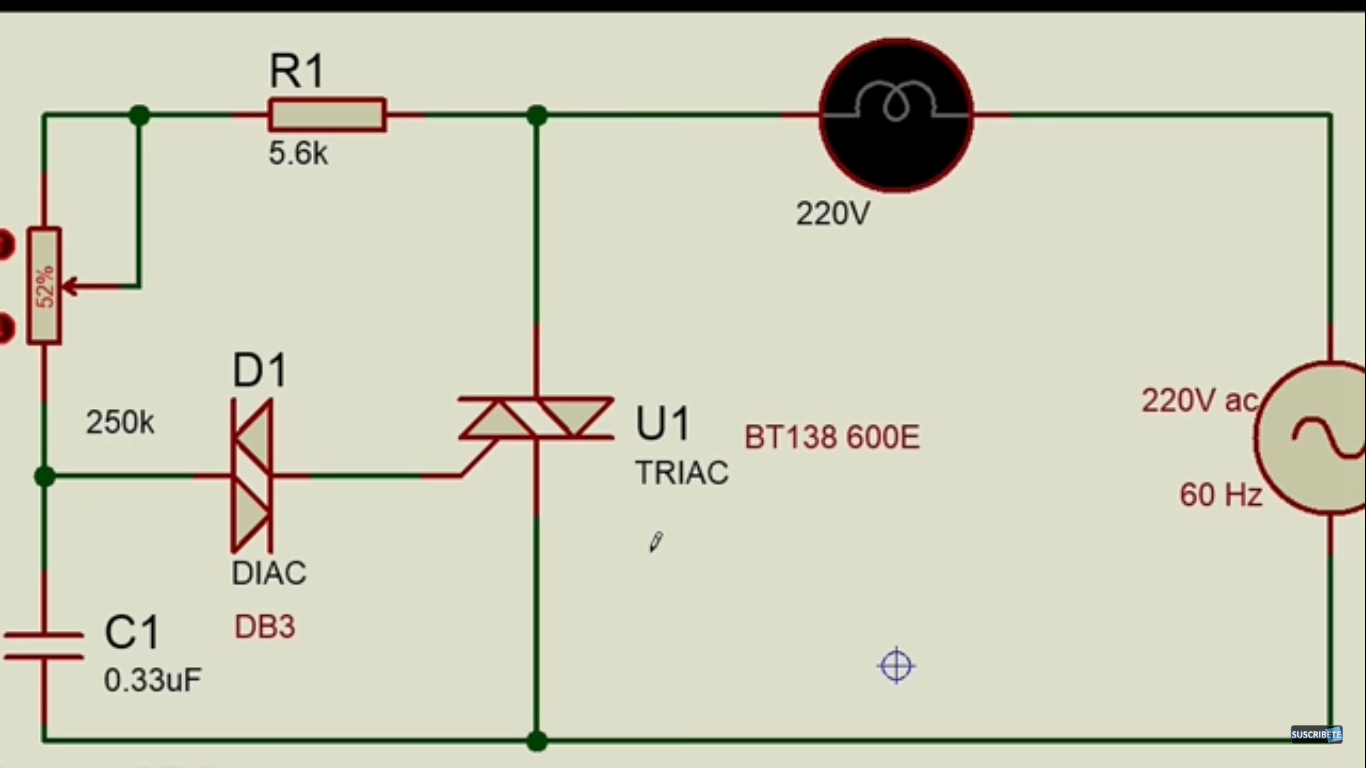
\includegraphics[scale=0.20]{/home/raulcb/Downloads/3.png}
\caption{.}
\label{.}
\end{figure}

\textbf{Este es el diagrama que seguimos para poder desarrollarlo.}
\\
Nos guiamos del esquemàtico que tenemos en la parte superior.
Empezamos con nuestra fuente. Para poder utilizarla tenemos una clavija conectada a un foco con uno de losextremos y el otro es el que va al circuito. Una de las linesa de la corriente alterna va conectado al pin 1 del TRIAC y asì mismo al capacitor, luego la otra linea va a uno de los bornes de la lampara, y del otro lado permite que fluya la corriente y es asì cuando llega a la resistencia fluye hacia la parte donde esta el diac, recordamos que eldiac es un dispositivo semiconductor, como los diodos, pero a diferencia del diodo, el diac permite controlareen ambas direcciones.
\\
Con este dispositivo podemos entender que deja que la corriente fluya y el TRIAC tenga su funcionamientto, pero aqui vemos de que manera funciona el diac, ya que este da pulsos de corriente, cada determinado tiempo deja psar una corriente positiva y otra negativa 
\\\\\\\\\\

\begin{figure}[htp]
\centering
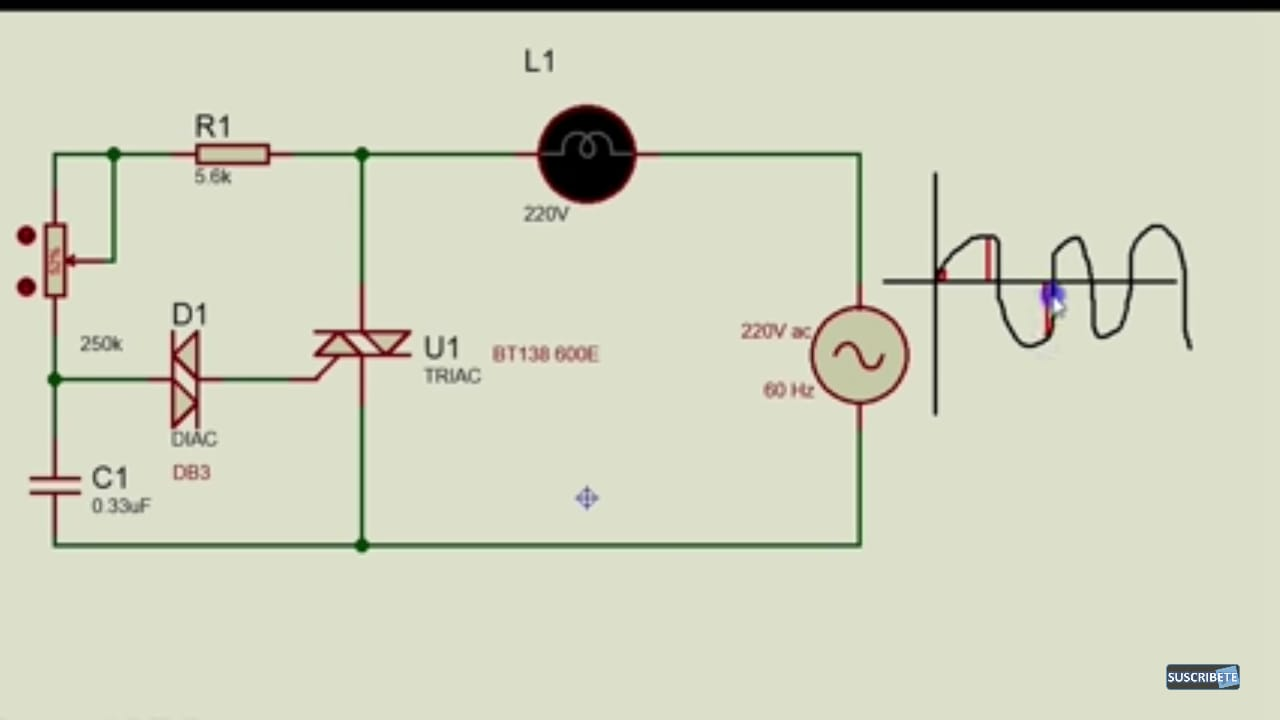
\includegraphics[scale=0.20]{/home/raulcb/Downloads/Diac.jpeg}
\caption{.}
\label{.}
\end{figure}

ES por ello que nos permite regular la intensidad luminosa.
\\

Pasamos a la parte del TRIAC.
En la parte del gate que es el pin 3, necesitamos activar con una corriente para poder conducir, es decir cuando una señal llega en esa parte, permite esl paso de la corriente, con lo cual se estaria cerrando el circuito, y es por ello que se enciende el foco.
\\
Ahora como es la regulaciòn, en un determinado tiempo manda una señal, cuando aumentamos el ohmiage de las resistencias es cuando pasa esto.
\section{Resusltado}
\begin{figure}[htp]
\centering
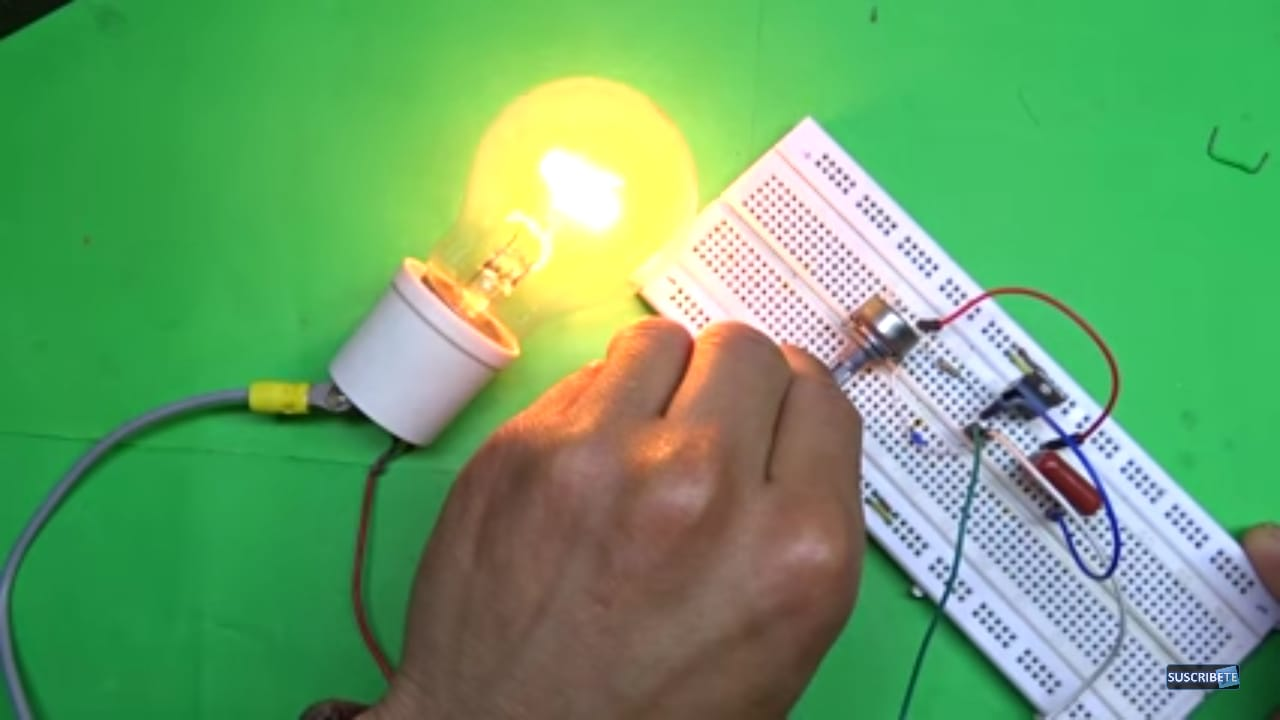
\includegraphics[scale=0.20]{/home/raulcb/Downloads/lll.jpeg}
\caption{.}
\label{.}
\end{figure}  

\section{Conclusiòn}
Es una pràctica sencilla que permite poder aprender como utilizar algo sencillo y como poder implementar en algo mas grande, ya que esto en la industria es algo de verdad nos ayudaria por montòn.





\end{document}
